
% \renewcommand\theequation{\thesection\arabic{equation}}
% \renewcommand\thefigure{\thesection\arabic{figure}}
% \setcounter{equation}{0}
% \setcounter{figure}{0}

\section{Derivation of the Likelihood Function}
\label{dga:sec:likelihood}

Here we provide a detailed derivation of our likelihood function (Eq.
\ref{dga:eq:likelihood}).
In its most general form, the problem at hand is to treat some set of data as a
stochasitc sample from an evolutionary track in some observed space.
This assumption implies that all of the data would fall perfectly on some
infinitely thin line or curve in the absence of measurement uncertainties.
We make no assumptions about the underlying model that computes the track, so
this approach should be universally applicable to one-zone GCE models of any
parametrization.
Evolutionary tracks also arise in the context of, e.g., stellar streams and
isochrones, indicating that our likelihood function should be easily extensible
to these models as well.
We however phrase our discussion here under the assumption that the observed
quantities are the abundances and ages of stars and that the underlying
framework is a one-zone GCE model (see discussion in~\S~\ref{dga:sec:onezone}).
\par
First, we define the key variables:
\begin{itemize}

	\item[\textbf{1.}] $\script{D} = \{\script{D}_1, \script{D}_2,
	\script{D}_3, ..., \script{D}_N\}$ is the data containing~$N$ individual
	stars with measurement uncertainties described by the covariance matrices
	of each datum~$C = \{C_1, C_2, C_3, ..., C_N\}$.
	The quantities associated with each star are not necessarily the same --
	that is, only some of the stars may have age measurements, or the
	abundances of some nuclear species may not be reliably measured for the
	whole sample.

	\item[\textbf{2.}] \script{M}~is the evolutionary track in chemical and age
	space.
	Although~\script{M} is a smooth and continuous curve in principle, in
	practice it is approximated in a piece-wise linear form computed by some
	numerical code.
	It can therefore also be expressed as a discrete set of~$K$ points
	$\script{M} = \{\script{M}_1, \script{M}_2, \script{M}_3, ...,
	\script{M}_K\}$ in the observed space connected by line segments.
	We demonstrate below that under this numerical approximation, the
	likelihood function for the continuous piece-wise linear track can be
	expressed as a summation over the discretely sampled points.

	\item[\textbf{3.}] $\{\theta\}$ is a chosen set of one-zone model
	parameters.
	These values impact the detailed form of the track~\script{M}~and otherwise
	affect the inferred best-fit values only if there is an assumed prior
	$L(\{\theta\})$ (see equation~\ref{dga:eq:bayes}).

\end{itemize}
\par
Given the track~\script{M}, the likelihood~$L(\script{D} | \{\theta\})$ of
observing the data can be expressed as the line integral of the differential
likelihood along~\script{M}:
\begin{equation}
L(\script{D} | \{\theta\}) = \int_\script{M} dL =
\int_\script{M} L(\script{D} | \script{M}) P(\script{M} | \{\theta\})
d\script{M},
\end{equation}
where~$P(\script{M} | \{\theta\})$ describes the probability that a singular
datum will be drawn from the model at a given point along the track.
The defining characteristic of the IPPP is that~$P(\script{M} | \{\theta\})$
follows a Poisson distribution~\citep{Press2007}:
\begin{equation}
P(\script{M}_j | \{\theta\}) = e^{-N_\lambda}
\prod_i^N \lambda (\script{M}_j | \{\theta\}),
\end{equation}
where for notational convenience below we leave the expression written as a
product over the~$N$ stars in the sample as opposed to~$\lambda^N$.
$\lambda$ is the~\textit{intensity function} describing the expected
number of stars at a specific point along the track~$\script{M}_j$.
$N_\lambda$ denotes the expected~\textit{total} number of stars in the sample
and can be expressed as the line integral of the intensity function along the
track:
\begin{equation}
N_\lambda = \int_\script{M} \lambda(\script{M} | \{\theta\}) d\script{M}.
\end{equation}
$\lambda$ describes the predicted~\textit{observed} distribution of stars in
chemical space and should therefore incorporate any selection effects in the
data.
It can be expressed as the product of the selection function~\script{S}~(see
discussion in~\S~\ref{dga:sec:fitting}) and the~\textit{intrinsic}
distribution~$\Lambda$ according to
\begin{equation}
\lambda(\script{M}_j | \{\theta\}) = \script{S}(\script{M}_j | \{\theta\})
\Lambda(\script{M}_j | \{\theta\}).
\end{equation}
Plugging the Poisson distribution into our expression for the likelihood
function, we obtain
\begin{subequations}\begin{align}
L(\script{D} | \{\theta\}) &= \int_\script{M}
\left(\prod_i^N L(\script{D}_i | \script{M})\right)
\left(e^{-N_\lambda} \prod_i^N \lambda(\script{M} | \{\theta\})\right)
d\script{M}
\\
&= e^{-N_\lambda} \prod_i^N \int_\script{M} L(\script{D}_i | \script{M})
\lambda(\script{M} | \{\theta\}) d\script{M},
\end{align}\end{subequations}
where we have exploited the conditional independence of each datum, allowing us
to substitute~$L(\script{D} | \script{M}) = \prod L(\script{D}_i |
\script{M})$.
We have also dropped the subscript~$j$ in~$\lambda(\script{M}_j | \{\theta\})$
because we are computing the line integral along the track~\script{M}, so a
specific location~$\script{M}_j$ is implicit.
\par
Now taking the logarithm of the likelihood function produces the following
expression for~$\ln L$:
\begin{equation}
\ln L(\script{D} | \{\theta\}) = -N_\lambda + \sum_i^N \ln \left(
\int_\script{M} L(\script{D}_i | \script{M})\lambda(\script{M} | \{\theta\})
d\script{M}
\right).
\label{dga:eq:lnL_with_integral}
\end{equation}
The next step is to assess the likelihood~$L(\script{D}_i | \script{M})$ of
observing each datum given the predicted track.
The line integral within the summation indicates that the most general solution
is to marginalize the likelihood over the entire evolutionary track.
In fact, we find in our tests against mock samples that this marginalizaion is necessary to
ensure that the inferred best-fit parameters are accurate (see discussion
in~\S~\ref{dga:sec:mocks:recovered}).
This requirement arises due to observational uncertainties -- there is no way
of knowing~\textit{a priori} which point on the track any individual datum is
truly associated with.
If this information were available,~$L(\script{D}_i | \script{M})$ would reduce
to a delta function at the known point~$\script{M}_j$.

\begin{figure}
\centering
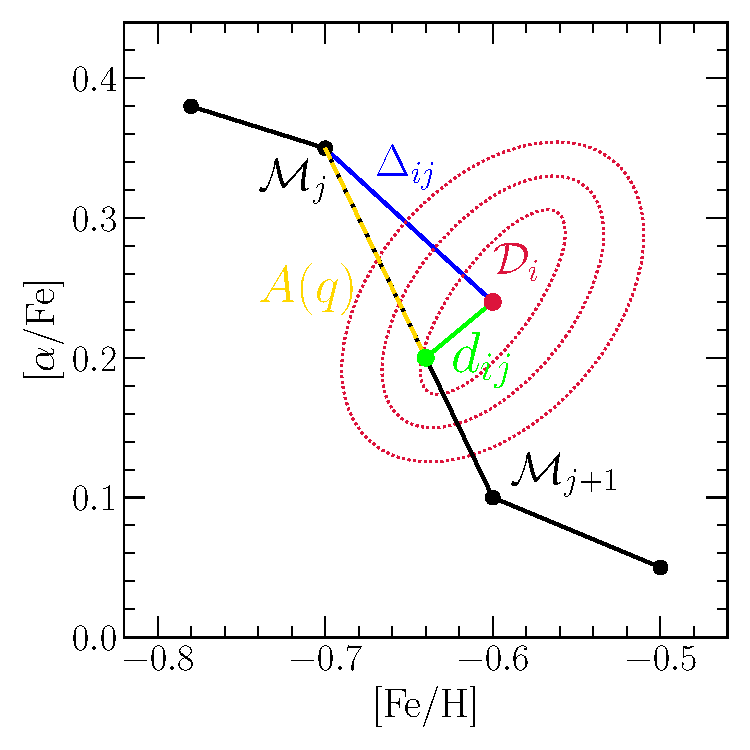
\includegraphics[scale = 0.6]{chapter3/derivation_cartoon.pdf}
\caption{
A schematic of our derivation and the quantities involved.
In practice, the evolutionary track~\script{M} is computed by some numerical
code as a piece-wise linear approximation -- here we exaggerate the spacing
between points for illustrative purposes.\tabularnewline
When the spacing~$\Delta\script{M}_j$ between the points~$\script{M}_j$ and
$\script{M}_{j + 1}$ is large compared to the observation uncertainties
associated with the datum~$\script{D}_i$ (shown by the dotted red contours),
the finite length of the line segment becomes an important correction.
Additional vector quantities that appear in our derivation are also noted.
}
\label{dga:fig:marginalization}
\end{figure}

In practice, the track may be complicated in shape and is generally not known
as a smooth and continuous function, instead in some piece-wise linear
approximation computed by a numerical code.
We visualize a hypothetical track and datum in Fig.~\ref{dga:fig:marginalization}
where we have deliberately exaggerated the spacing between two adjacent
points~$\script{M}_j$ and~$\script{M}_{j + 1}$ for illustrative purposes.
In principle, the likelihood of observing some datum~$\script{D}_i$ varies
along the line segment~$\Delta\script{M}_j$ connecting the two points.
To properly take this variation into account, we must integrate along the
length of the line segment:
\begin{equation}
L(\script{D}_i | \script{M}_j) = \int_0^1 L(\script{D}_i | \script{M}_j, q) dq,
\label{dga:eq:l_int_q}
\end{equation}
where~$q$ is a dimensionless parameter defined to be 0 at the point
$\script{M}_j$ and 1 at the point~$\script{M}_{j + 1}$ according to
\begin{equation}
A(q) = \script{M}_j + q(\script{M}_{j + 1} - \script{M}_j)
= \script{M}_j + q\Delta\script{M}_j.
\end{equation}
If the errors associated with the observed datum~$\script{D}_i$ are accurately
described by a multivariate Gaussian, then the likelihood of observing
$\script{D}_i$ given a point along this line segment can be expressed in terms
of its covariance matrix~$C_i$ as
\begin{subequations}\begin{align}
L(\script{D}_i | \script{M}_j, q) &=
\frac{1}{\sqrt{2\pi \det{(C_i)}}}
\exp\left(\frac{-1}{2} d_{ij}(q) C_i^{-1} d_{ij}^T(q)\right)
\label{dga:eq:l_di_mj_q}
\\
d_{ij} &= \script{D}_i - A(q)
\\
&= \script{D}_i - \script{M}_j - q(\script{M}_{j + 1} - \script{M}_j)
\\
&= \Delta_{ij} - q\Delta \script{M}_j,
\label{dga:eq:delta_minus_qmj}
\end{align}\end{subequations}
where~$d_{ij}$ is the vector difference between~$\script{D}_i$ and the
point along the track~$A(q)$ in the observed space.
For notational convenience, we have introduced the variable
$\Delta_{ij} = \script{D}_i - \script{M}_j$ as the vector difference between
the~$i$th datum and the~$j$th point sampled on the track.
We clarify our notation that the subscripts~$i$ and~$ij$ in equation
\refp{dga:eq:l_di_mj_q} above do not refer to rows and columns of matrices, but
rather to the~$i$th datum and the~$j$th point on the model track.
If a multivariate Gaussian is not an accurate description of the measurement
uncertainties in any one datum, then equation~\refp{dga:eq:l_di_mj_q} must
be replaced with some alternative characterization of the likelihood of
observation, such a kernel density estimate evaluated at the point~$A(q)$.
We however continue our derivation under the assumption of multivariate
Gaussian uncertainties.
\par
Before evaluating equation~\refp{dga:eq:l_int_q}, we first compute the square
$d_{ij}(q)C_i^{-1}d_{ij}^T(q)$ and isolate the terms that depend on~$q$:
\begin{subequations}\begin{align}
\begin{split}
d_{ij}(q) C_i^{-1} d_{ij}(q)^T &= \Delta_{ij} C_i^{-1} \Delta_{ij}^T -
2q\Delta_{ij}C_i^{-1}\Delta \script{M}_j^T +
\\
&\qquad q^2\Delta \script{M}_j C_i^{-1} \Delta \script{M}_j^T
\end{split}
\label{dga:eq:chisquared}
\\
&= \Delta_{ij} C_i^{-1} \Delta_{ij}^T - 2bq + aq^2,
\end{align}\end{subequations}
where we have introduced the substitutions
$a = \Delta\script{M}_j C_i^{-1} \Delta\script{M}_j^T$ and
$b = \Delta_{ij} C_i^{-1} \Delta\script{M}_j^T$.
Plugging this expression into the exponential in equation~\refp{dga:eq:l_di_mj_q}
and integrating from~$q = 0$ to~$1$ according to equation~\refp{dga:eq:l_int_q}
yields the following expression for~$L(\script{D}_i | \script{M}_j)$:
\begin{subequations}\begin{align}
\begin{split}
L(\script{D}_i | \script{M}_j) &= \frac{1}{\sqrt{2\pi \det{(C_i)}}}
\exp\left(\frac{-1}{2}\Delta_{ij} C_i^{-1} \Delta_{ij}^T\right)
\\
&\qquad \int_0^1 \exp\left(\frac{-1}{2}(aq^2 - 2bq)\right)dq
\end{split}
\\
\begin{split}
&= \frac{1}{\sqrt{2\pi\det{(C_i)}}}
\exp\left(\frac{-1}{2}\Delta_{ij}C_i^{-1}\Delta_{ij}^T\right)
\sqrt{\frac{\pi}{2a}}
\\
&\qquad \exp\left(\frac{b^2}{2a}\right)
\left[\erf\left(\frac{a - b}{\sqrt{2a}}\right) - \erf\left(\frac{b}{\sqrt{2a}}
\right)\right].
\end{split}
\end{align}\end{subequations}
For notational convenience, we introduce the corrective term~$\beta_{ij}$ given
by
\begin{equation}
\beta_{ij} = \sqrt{\frac{\pi}{2a}} \exp\left(\frac{b^2}{2a}\right)
\left[\erf\left(\frac{a - b}{\sqrt{2a}}\right) - \erf\left(\frac{b}{\sqrt{2a}}
\right)\right],
\label{dga:eq:corrective_beta}
\end{equation}
such that~$L(\script{D}_i | \script{M}_j)$ can be expressed as
\begin{equation}
L(\script{D}_i | \script{M}_j) = \frac{\beta_{ij}}{\sqrt{2\pi \det{(C_i)}}}
\exp\left(\frac{-1}{2}\Delta_{ij} C_i^{-1} \Delta_{ij}^T\right).
\end{equation}
With this expression for the likelihood~$L(\script{D}_i | \script{M}_j)$ of
observing the datum~$\script{D}_i$ marginalized over the length of the line
segment~$\Delta\script{M}_j$,~$L(\script{D}_i | \script{M})$ can now be
written a summation over each individual line segment.
As mentioned above, the numerical piece-wise linear approximation of the smooth
and continuous form reduces to a summation over the individual points
$\script{M} = \{\script{M}_1, \script{M}_2, \script{M}_3, ..., \script{M}_K\}$
at which the track is sampled:
\begin{equation}\begin{split}
&\ln L(\script{D} | \{\theta\}) = -N_\lambda
- \sum_i^N \ln \left(\sqrt{2\pi \det{(C_i)}}\right) +
\\
&\qquad \sum_i^N \ln \left(
\sum_j^K \beta_{ij}
\exp\left(\frac{-1}{2}\Delta_{ij}C_i^{-1}\Delta_{ij}^T\right)
\lambda(\script{M}_j | \{\theta\})
\right).
\end{split}\end{equation}
Although we have exaggerated the spacing between points for illustrative
purposes, Fig.~\ref{dga:fig:marginalization} indicates that
$q\Delta\script{M}_j \ll \Delta_{ij}$ in the opposing case in which
$\Delta\script{M}_j$ is small compared to the measurement uncertainties.
As a consequence,~$\beta_{ij} \approx 1$ and this corrective term can be safely
neglected.
In some cases, however, computing the evolutionary track~\script{M}~may be
computationally expensive, making it potentially advantageous to reduce the
the number of computed points~$K$ in exchange for a slightly more complicated
likelihood calculation.
\par
As discussed above, the intensity function~$\lambda$ quantifies the observed
density of points, incorporating any selection effects present in the data into
the predicted intrinsic density~$\Lambda$.
In a one-zone GCE model,~$\Lambda$ is given by the SFR at the point
$\script{M}_j$ (to incorporate the effects dying stars or stars at a given
evolutionary stage, one can modify the selection function~\script{S}).
This multiplicative factor on the likelihood~$L$ can be incorporated by simply
letting the pair-wise component of the datum~$\script{D}_i$ and the point along
the track~$\script{M}_j$ take on a weight
$w_j \equiv \script{S}(\script{M}_j | \{\theta\}) \dot{M}_\star(\script{M}_j |
\{\theta\})$ determined by the survey selection function~\script{S}~and the
SFR~$\dot{M}_\star$ at the point~$\script{M}_j$.
The predicted number of instances~$N_\lambda$, originally expressed as the
line integral of~$\lambda$, can now be expressed as the sum of the
weights~$w_j$.
The following likelihood function then arises:
\begin{equation}
\ln L(\script{D} | \{\theta\}) \propto
\sum_i^N \ln \left(\sum_j^K
\beta_{ij} w_j \exp\left(\frac{-1}{2}\Delta_{ij} C_i^{-1} \Delta_{ij}^T\right)
\right) - \sum_j^K w_j,
\label{dga:eq:lnL_minus_weights}
\end{equation}
where we have omitted the term~$\sum \ln \left(\sqrt{2\pi \det{(C_i)}}\right)$
because it is a constant that can safely be neglected in the interest of
optimization.
This likelihood function considers each pair-wise combination of the data and
model, weighting the likelihood according to the predicted density of
observations and penalizing models by the sum of their weights.
This term can also be described as a reward for models that explain the
observations in as few predicted instances as possible.
\par
In many one-zone GCE models, however, the normalization of the SFH is
irrelevant to the evolution of the abundances.
Because the metallicity is given by the metal mass~\textit{relative} to the ISM
mass, the normalization often cancels.
Because the SFH determines the weights, it is essential in these cases to
ensure that the sum of the weights has no impact on the inferred likelihood.
To this end, we consider a density~$\rho$ with some unknown overall
normalization defined relative to the intensity function according to
\begin{subequations}\begin{align}
\lambda(\script{M} | \{\theta\}) &= N_\lambda \rho(\script{M} | \{\theta\})
\\
\int_\script{M} \rho(\script{M} | \{\theta\}) d\script{M} &= 1.
\end{align}\end{subequations}
Plugging~$\rho$ into equation~\refp{dga:eq:lnL_with_integral} and pulling
$N_\lambda$ out of the natural logarithm yields the following expression:
\begin{equation}\begin{split}
\ln L(\script{D} | \{\theta\}) &= -N_\lambda + N \ln N_\lambda +
\sum_i^N \ln \left(\sqrt{2\pi \det{(C_i)}}\right) +
\\
&\qquad \sum_i^N \ln \left(
\int_\script{M} L(\script{D}_i | \script{M}) \rho(\script{M} | \{\theta\})
d\script{M} \right).
\end{split}\end{equation}
With~$\rho$ in place of~$\lambda$ and the extra term~$N \ln N_\lambda$,
reducing this equation proceeds in the exact same manner as above, resulting
in the following likelihood function:
\begin{equation}\begin{split}
\ln L(\script{D} | \{\theta\}) &= -N_\lambda + N \ln N_\lambda +
\sum_i^N \ln \left(\sqrt{2\pi \det{(C_i)}}\right) +
\\
&\qquad \sum_i^N \ln \left(
\sum_j^K \beta_{ij} w_j
\exp\left(\frac{-1}{2}\Delta_{ij} C_i^{-1} \Delta_{ij}^T\right)\right).
\end{split}\end{equation}
For notational convenience, we have left the normalization of the weights
written as~$N_\lambda$.
In the interest of optimizing the likelihood function, we take the partial
derivative of~$\ln L$ with respect to~$N_\lambda$ and find that it is equal to
zero when~$N_\lambda = N$.
Because~$\rho$ is by definition un-normalized, we can simply choose this
overall scale (this is also the ``most correct'' scale in the sense that the
number of stars in the sample is exactly as predicted).
The first two terms in the above expression for~$\ln L$ then become
$-N + N \ln N$, a constant for a given sample which can safely be neglected
for optimization along with the term incorporating the determinants of the
covariance matrices.
We arrive at the following expression for the likelihood function in cases
where the normalization of the SFH does not impact the evolution of the
abundances:
\begin{subequations}\begin{align}
\ln L(\script{D} | \{\theta\}) &\propto \sum_i^N \ln \left( \sum_j^K \beta_{ij}
w_j \exp\left(\frac{-1}{2}\Delta_{ij} C_i^{-1} \Delta_{ij}^T\right) \right)
\label{dga:eq:lnL_fracweight}
\\
\sum_j^K w_j &= 1,
\label{dga:eq:lnL_fracweightsum}
\end{align}\end{subequations}
where the second expression arises from the requirement that the line integral
of the un-normalized density~$\rho$ along the track equal 1.
\par
In summary, when inferring best-fit parameters for one-zone GCE models in which
the normalization of the SFH is irrelevant to the evolution of the abundances,
authors should adopt equations~\refp{dga:eq:lnL_fracweight} and
\refp{dga:eq:lnL_fracweightsum}.
If the model is instead parametrized in such a manner that the normalization
does indeed impact the abundance evolution, then authors should adopt
equation~\refp{dga:eq:lnL_minus_weights}.
Such models can arise, e.g., when the mass-loading factor~$\eta$ grows with the
stellar mass to mimic the deepending of the potential
well~\citep[e.g.,][]{Conroy2022}.
In either case, the corrective term~$\beta_{ij}$ given by equation
\refp{dga:eq:corrective_beta} is approximately 1 and can be safely neglected when
the track is densely sampled relative to the observational uncertainties.
In the present paper, our GCE models are parametrized in such a manner that the
normalization of the SFH does~\textit{not} impact the enrichment history, and
we adopt equations~\refp{dga:eq:lnL_fracweight} and~\refp{dga:eq:lnL_fracweightsum}
accordingly.

